%%%Preamble
\documentclass[12pt]{article}
\usepackage{epsfig, amsfonts, cite, amssymb}
\usepackage{subfigure}
\usepackage{array}
\usepackage{float}
\usepackage{enumitem}
\usepackage{indentfirst}
\usepackage{boldline}
\usepackage[usenames,dvipsnames,svgnames,table]{xcolor}
\usepackage{amsmath}

%%% Use these when running Text Verifications
%\usepackage[T1]{fontenc}        
%\usepackage[utf8]{inputenc}     
%\usepackage[adobe-utopia]{mathdesign}
%\usepackage{printlen}

\voffset=0in \hoffset=0in \textwidth=6.3in \textheight=8.3in
\setlength{\oddsidemargin}{0in} \setlength{\textwidth}{6 in}
\thispagestyle{empty}

\begin{document}

\begin{figure*}[htb]
\subfigure{
\includegraphics[width=2.5in]{wne.eps} }
\hfil \hspace{.5in}
\subfigure{
\includegraphics[width=2.5in]{department.eps} }
\end{figure*}

%%%Header
\begin{center}
{\Large {\bf CPE 462/562 VHDL: Simulation \& Synthesis}}\\
\vspace{0.2in}
{\Large{Midterm Project: 4-bit ALU Design and Implementation}} \\
\vspace{0.2in}

%%%Cover Page
Katelyn Charbonneau\\
Email: kc325844@wne.edu\\
Date: 10/27/2017\\
\end{center}

\begin{table}[!h]
\centering
\begin{tabular}{| >{\arraybackslash}m{4in} | >{\centering\arraybackslash}m{1in} | }
  \hline
  % after \\: \hline or \cline{col1-col2} \cline{col3-col4} ...
  \textbf{Tasks} & \textbf{Grades} \\
  \hline
  &\\
  Task 1. Design, test, and verify 4-bit ALU (50') & \\
  &\\
  \hline
  &\\
  Task 2. Program DE2-115 and demonstrate 4-bit ALU (10') & \\
  &\\
  \hline
  &\\
  Task 3. Display INPUT and OUTPUT decimal equivalent values on SSDs (20') & \\
  &\\
  \hline
  &\\
  Report (20') & \\
  &\\
  \hline
    &\\
  Bonus (10') & \\
  &\\
  \hline
  \hline
    &\\
  \textbf{Total (100/110):} & \\
  &\\
  \hline

\end{tabular}
\label{table_cover}
\end{table}

%%% END of Cover Page
\newpage

\section{Objective} \label{sec:obj}
The objectives of the project are to be familiar with behavioral architecture; be able
to write a behavioral VHDL code to design a 4-bit arithmetic logic unit (ALU), write
a testbench to verify the design, and implement the ALU on FPGA.

\section{Design Procedure} \label{sec:desproc}
While testing of this design was done using a 4-bit bus width, their sizes are really defined as generics.  Thus, there is a variable bus size.  As part of this project, a ripple carry adder (RCA) is needed.  A fixed 4-bit width RCA design was available and was edited to also allow for a variable bus width.  This design was tested using a 6-bit width; sample results are in Section \ref{simresults}.	A block diagram for this is shown in Figure \ref{fig:rca}.

\begin{figure}[H]
\begin{center}
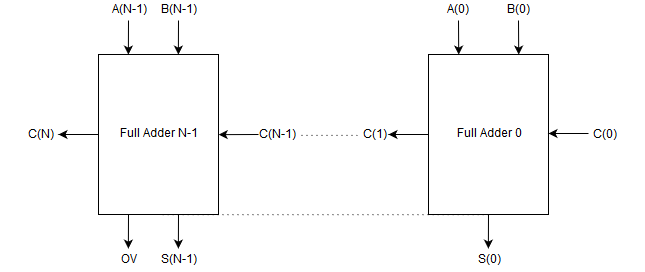
\includegraphics[scale=0.6]{Scalable_rca.png}
\caption{The RCA used to perform arithmetic calculations}
\label{fig:rca}
\end{center}
\end{figure}

Where N is the bus width, A, B, and S (sum) are vectors of length N-1, C (carry) is a vector of length N, and OV is defined as C(N) $\oplus$ C(N-1).

\newpage

The operations that the ALU can perform, as listed in the project requirements, are listed below:

\begin{table}[!h]
\vspace{0.1in}
\centering
	\rowcolors{2}{gray!10}{white}
	\begin{tabular}{ c  c  c  c} %\cline{2-7}
	\hlineB{4}
	\rowcolor{gray!25}
	\textbf{F\textunderscore BUS} & \textbf{C\textunderscore BUS} & \textbf{CBout} & OVERFLOW\\\hlineB{4}
	000 & A\textunderscore BUS & PASS & 0\\\hline
	001 & A\textunderscore BUS + B\textunderscore BUS + CBin & CBout & Overflow \\\hline
	010 & A\textunderscore BUS - B\textunderscore BUS - CBin & CBout & Overflow\\\hline
	011 & A\textunderscore BUS OR B\textunderscore BUS & PASS & 0\\\hline
	100 & A\textunderscore BUS XOR B\textunderscore BUS & PASS & 0\\\hline
	101 & A\textunderscore SRA 3 & PASS & 0\\\hline
	110 & A\textunderscore BUS SLL 2 & A\textunderscore BUS(N-1) & Overflow\\\hline
	111 & A\textunderscore BUS ROR -3 & PASS & 0\\\hlineB{4}
	\end{tabular}
\label{tab:results1}
\caption{ALU Operations}
\end{table}

The RCA is used in cases 1 and 2 - addition and subtraction.  All other cases are handled by simple pre-defined operations within VHDL.  Note that there is overflow for case 6 if the value of A\textunderscore Bus(N-1) changes after shifting.

\newpage

\section{Simulation Results} \label{simresults}
\begin{figure}[H]
\begin{center}
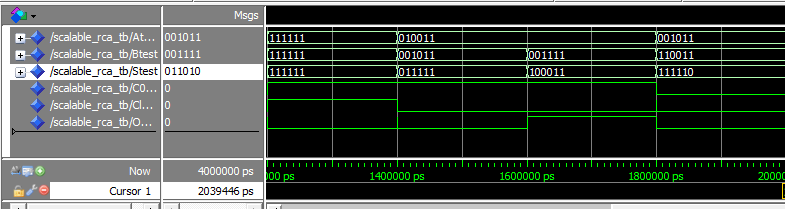
\includegraphics[scale=0.7]{rca_sim_results_example.png}
\caption{A few example operations on the RCA design using 6 bits}
\label{fig:simrca0}
\end{center}
\end{figure}

\section{Demonstration on FPGA} \label{demo}
pictures of on board demo and discussions...
 
\section{Conlusion} \label{cncl}
your conclusion goes here...

\end{document} 
